%%% lorem.tex --- 
%% 
%% Filename: lorem.tex
%% Description: 
%% Author: Ola Leifler
%% Maintainer: 
%% Created: Wed Nov 10 09:59:23 2010 (CET)
%% Version: $Id$
%% Version: 
%% Last-Updated: Wed Nov 10 09:59:47 2010 (CET)
%%           By: Ola Leifler
%%     Update #: 2
%% URL: 
%% Keywords: 
%% Compatibility: 
%% 
%%%%%%%%%%%%%%%%%%%%%%%%%%%%%%%%%%%%%%%%%%%%%%%%%%%%%%%%%%%%%%%%%%%%%%
%% 
%%% Commentary: 
%% 
%% 
%% 
%%%%%%%%%%%%%%%%%%%%%%%%%%%%%%%%%%%%%%%%%%%%%%%%%%%%%%%%%%%%%%%%%%%%%%
%% 
%%% Change log:
%% 
%% 
%% RCS $Log$
%%%%%%%%%%%%%%%%%%%%%%%%%%%%%%%%%%%%%%%%%%%%%%%%%%%%%%%%%%%%%%%%%%%%%%
%% 
%%% Code:


\chapter{Method}
This chapter will summarize and describe the methods and approaches used to answer the problems stated in \textit{Section 1.3}. The first section will describe the workflow proposed to generate the final results. The second section describes how the results will be evaluated.

\section{Implementation}
\noindent The work will be implemented in steps described in \textit{Figure \ref{fig:method workflow}}. Each step is dependent on the output of its predecessor. The first step is to identify and mask the agar plate. With the irrelevant data masked, the second step is to identify the compartment edges in the agar plate. With the agar plate and its compartment edges identified, the orientation will be calculated based on the output of the previous steps. Lastly, based on gathered key points, the images will be processed using image registration. \\

\begin{figure}[H]
    \centering
     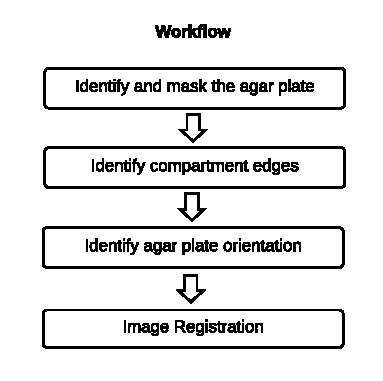
\includegraphics[width=.43\linewidth]{figures/PDF/Workflow.pdf}\\
    \caption{Workflow of the implementation structure}
    \label{fig:method workflow}
\end{figure}

\subsection{Identify and mask the agar plate}
The first step is to identify the agar plate, which will provide an elliptical contour of points that defines the ROI. The workflow will be structured, as shown in \textit{Figure \ref{fig:identify and mask flowchart}}, and described throughout the section. 
\begin{figure}[H]
    \centering
    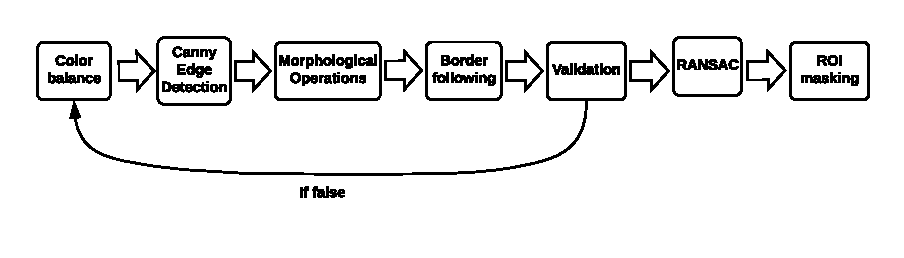
\includegraphics[width=1\linewidth]{figures/PDF/Identify and mask agar plate.pdf}\\
    \caption{Flowchart to identify and mask the agar plate.}
    \label{fig:identify and mask flowchart}
\end{figure}

%\noindent \textbf{Color balance} \\
%\noindent \color{red} Describe the brightness and contrast algorithm in the Theory section. \color{black} 

\noindent Different images might not have the same conditions regarding the illumination or intensity of RGB values, which means that each image might not get the same result when being processed.  Therefore, it is essential to even out these variables. However, images that are too dark or too bright may not take full advantage of color balancing; they may also need to balance brightness and intensity beforehand.  Each input will, therefore, be processed in terms of balancing brightness and contrast, followed by color balancing using SCB before further processing. The goal of this step is to improve the accuracy of the final output. \\

%\noindent\textbf{Canny, Thresh, Morph}\\
\noindent With contrast, brightness, and color all balanced, the next step is to process the image using Canny to intensify edges and reducing any image noise. Before applying Canny, an additional Gaussian blur will firstly be applied to reduce any bacteria within each compartment. Configuring Canny to the desired level with a minimal number of bacteria clusters, however, might cause disconnectivity in the outer contour. Morphological operations such as Closing will then be used to repair any broken lines. \\ 


\noindent The next step is to define any contours. CHT could be used to identify a perfectly circular contour, but due to variations in perspective, the agar plate will always be a bit elliptical. Using CHT, in this case, would give inaccurate results. Therefore, the contour will be found using border following. The contour found in the highest hierarchy should represent the external contour of the agar plate. However, some segments of the contour may, in some cases,  be imperfect due to, e.g., bacteria clusters growing close to the edge. The contour will, therefore, be fitted to an elliptical model using RANSAC, which should give a better approximation of the external contour, providing the desired set of key-points.  
%\\\color{red} “Mention in the Theory chapter that contours a sorted in hierarchies.” \color{black}  \\


\noindent Each image will be validated before proceeding to the final step of this section. The contour defined with conic fitting will then be compared with an approximated contour found using CHT. The comparison will be made using Hu Moments. Since the conic fitting contour will be elliptical and the contour from CHT always will be circular, a margin of error will be considered. If the Hu Moment returns a value exceeding the margin of error, the whole workflow process will be repeated. Invalid matches may be the result of bacteria clusters covering segments of the agar plate edges in shadowed areas. However, the problem can be solved by increasing or decreasing the initial brightness or contrast. The image will be reprocessed until a valid match is found. \\  

\noindent Lastly, with the ROI defined by the contour key-points from previous steps, a binary mask will be applied to the image, removing the unwanted background.\\


\subsection{Identify compartment edges}
\noindent The second process is to identify the compartment edges and the center point on the agar plate. Each compartment divider can be segmented as two straight lines i.e., compartment edges. Therefore, by using Hough Transform, these shapes can be identified. However, some pre-processing is needed to identify the edges correctly and reduce irrelevant noise that might occur. \textit{Figure \ref{fig:compartment edges flowchart} } illustrates how the workflow is structured. \\


\begin{figure}[H]
    \centering
     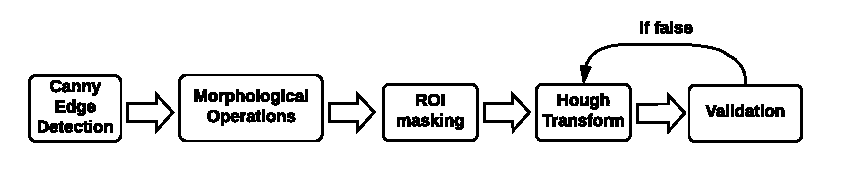
\includegraphics[width=0.9\linewidth]{figures/PDF/Identify compartment edges.pdf}\\
    \caption{Workflow to identify the compartment edges and the center point of the agar plate.}
    \label{fig:compartment edges flowchart}
\end{figure}

\noindent Once again, Canny, with an extra Gaussian blur, is applied to identify only the most distinct edges. The difference in this case, compared to finding the outer contour, is that only the centermost line of the compartment edges is of interest. As seen in \textit{Figure \ref{fig:compartment masking} b)}, each compartment divider consists of two edges, one on each side. Finding the centermost line is important since the intersection between the two crossing compartment edges constitutes the actual center point of the agar plate. The edges of each side of each compartment division can be merged to form one thick line using Morphological Closing. By using Skeletonize, the line can then be reduced to represent a pixel-wide centerline of each divider. \\

\noindent The mask boundaries from the previous section will be reused. The mask will be reduced in size, leaving a new ROI. As shown in \textit{Figure \ref{fig:compartment masking} a)}, the area outside the drawn boundary is not needed to identify the positioning and angle of the compartment edges, and should, therefore, be masked. \\


\begin{figure}[H]
    \centering
    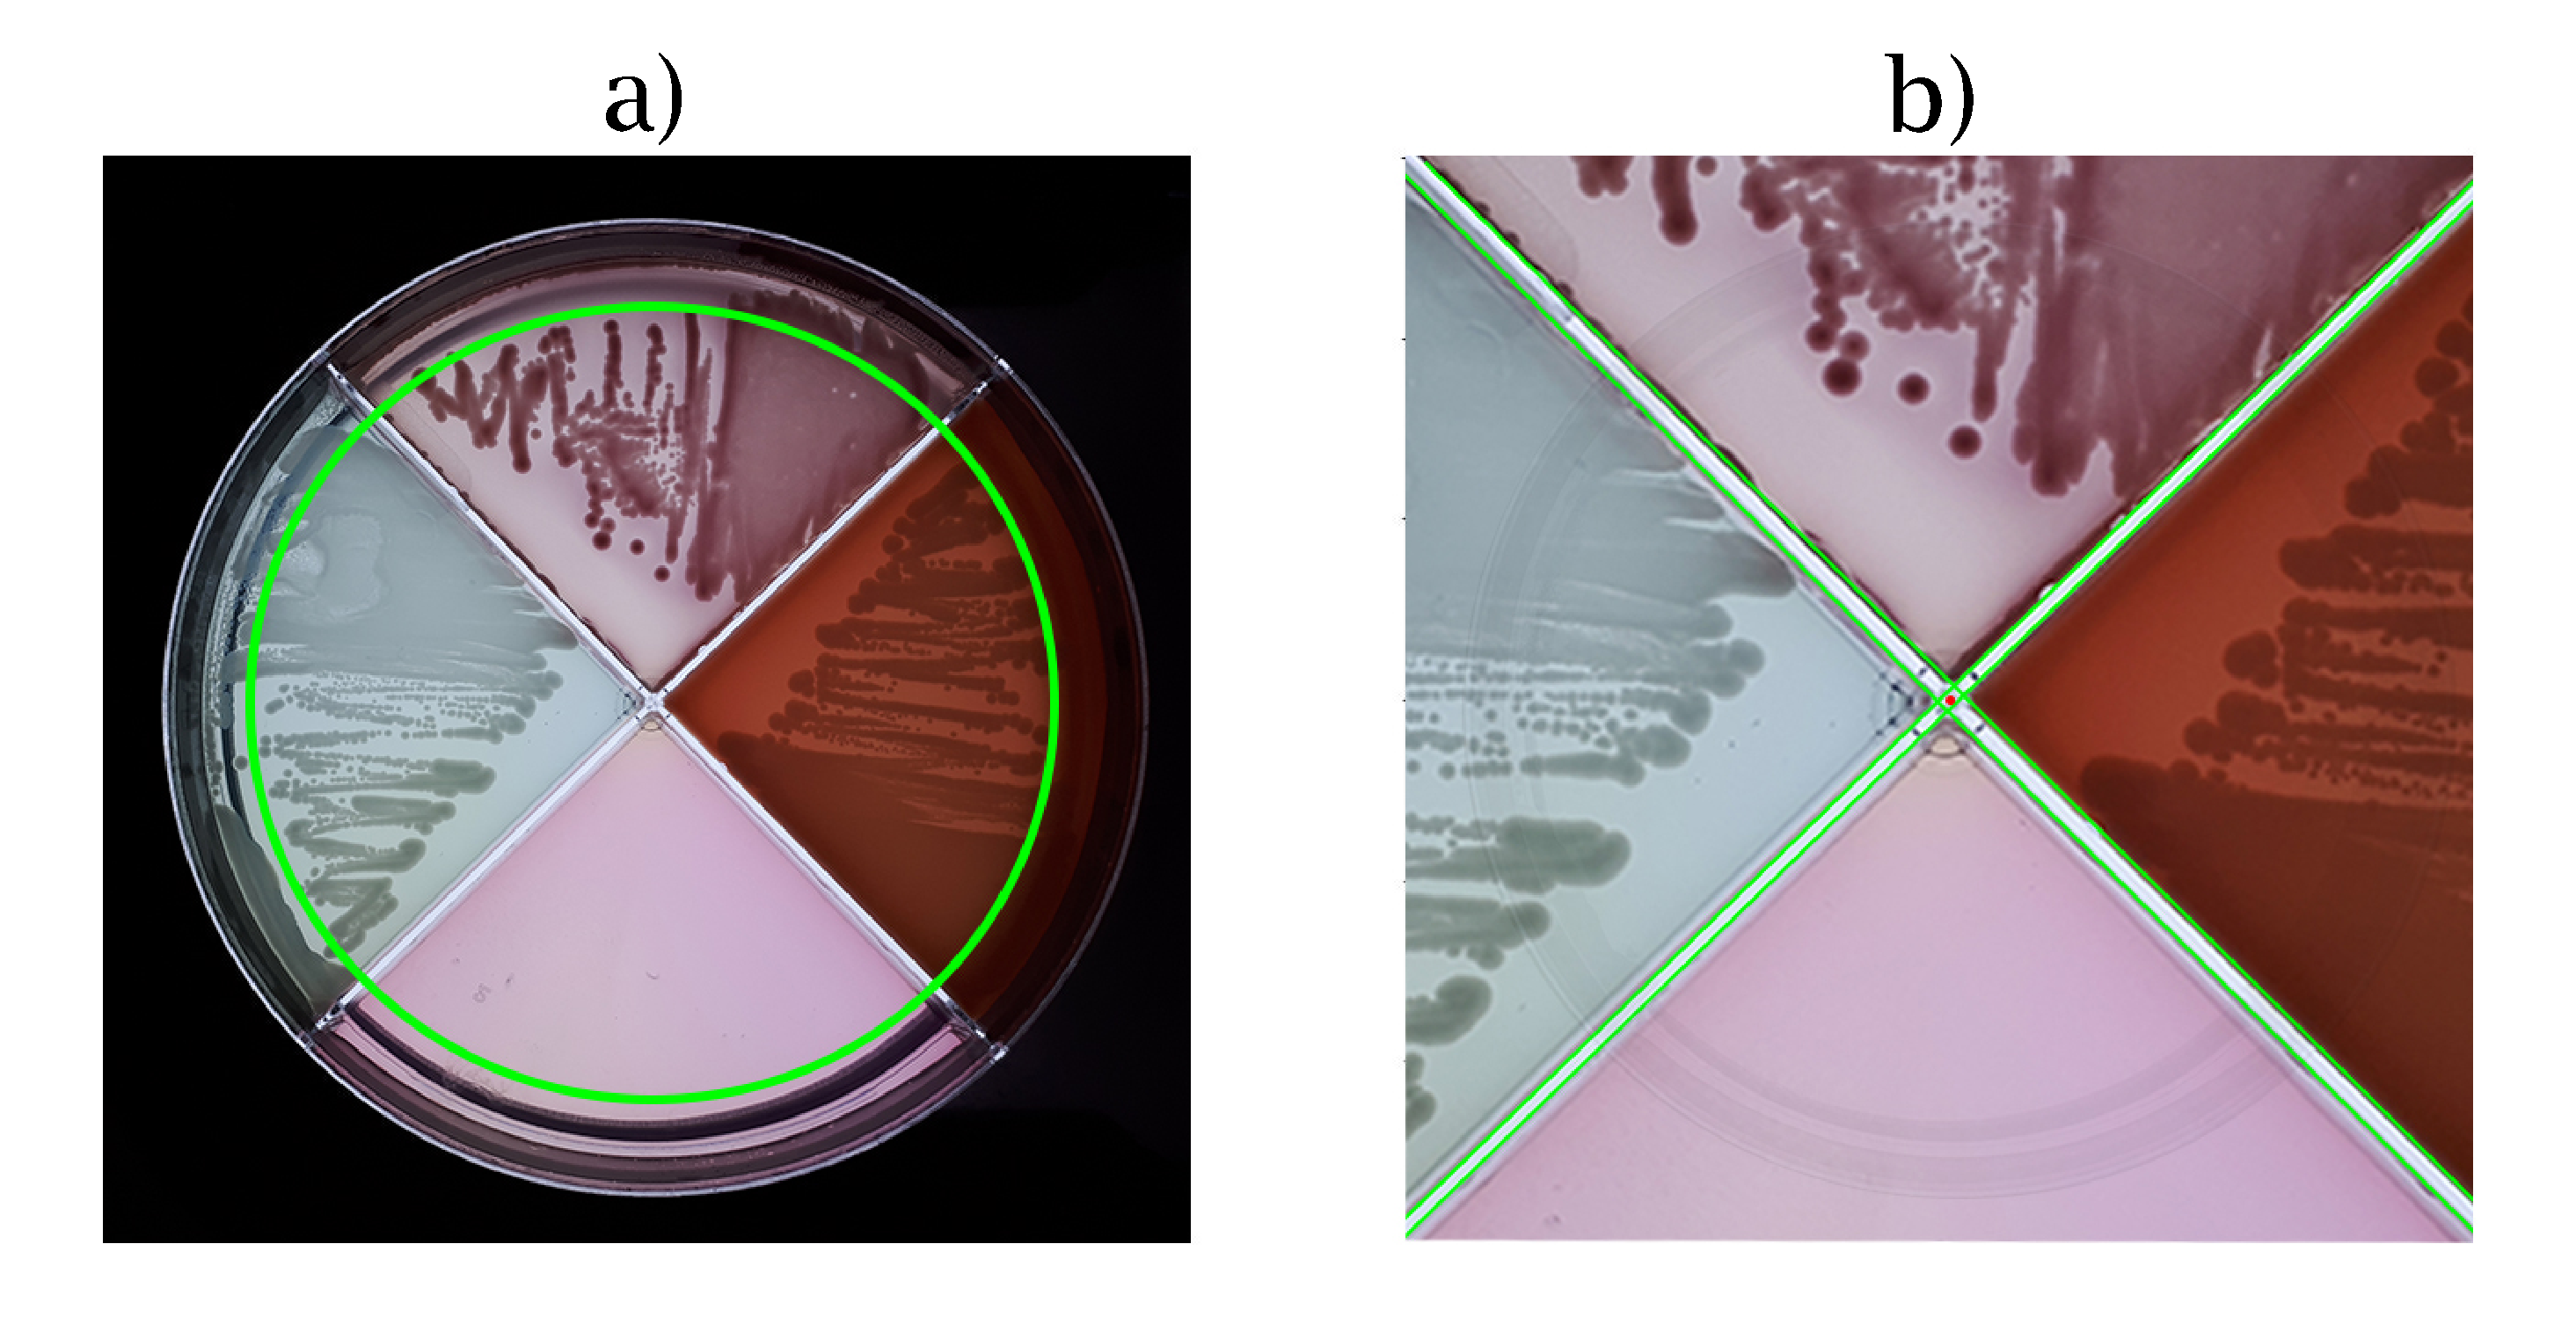
\includegraphics[width=.8\linewidth]{figures/PDF/ROI_boundaries.pdf} \\
    \caption{a) illustrates the new ROI boundary. b) show the edges and intersection (i.e., center point) of the compartment edges.}
    \label{fig:compartment masking}
\end{figure}

\noindent With a binary image representing the skeleton of the compartment edges, Hough Transform is used to identify the skeleton as lines. Lines will be sorted and validated in pairs based on values of rho and theta to make sure that only one line in each direction of the dividers is found. \\

\subsection{Identify agar plate orientation}
This part will focus on how to detect the rotation of the agar plate using segmentation. As shown in \textit{Figure \ref{fig:orientation flowchart}}, color space segmentation will be used to define the agar plate orientation, and key-points extracted from the previous sections can lastly be sorted considering rotation.\\ 
 
 \begin{figure}[H]
     \centering
      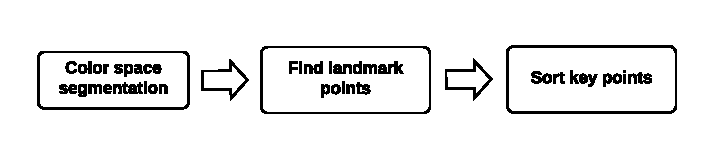
\includegraphics[width=0.7\linewidth]{figures/PDF/Identify agar plate orientation.pdf}\\
     \caption{Flow chart to identify the orientation of the agar plate.}
     \label{fig:orientation flowchart}
 \end{figure}


\noindent In the image dataset, the red compartment found in each image stands out. Since any compartments within an agar plate typically need to be distinguishable to the human eye,  color-based landmarks could be generally assumed here. The location of the segmented compartment will then be used to calculate the orientation.\\

\noindent Selecting the most prominent color should result in the most accurate output. The first step is to analyze both the HSV- and RGB-space of the image, generating corresponding 3D scatter plots of their color space. The color space providing the most visually separable and localized tones of red should be chosen. From the color space chosen, values from the scatter plot can be read to apply approximated values to the image.\\

\noindent With the selected compartment segmented, the intersection points between the outer contour in \textit{Section 4.1.1} and the lines from \textit{Section 4.1.2} are calculated as a first step to find the landmark points. Pixels on a line between each intersection point will be checked clockwise, forming a rectangular bounding box. A mean value of the pixel intensity on each line will be calculated. The line with the highest mean value should be the one crossing the segmented compartment, and the start- and end coordinate of the line will then define the first two landmark points. Remaining two intersection points will then be sorted clockwise in ascending order. From the sorted intersection point, all key-points from the previous two sections will lastly be sorted considering the rotation.


\subsection{Image registration}
The final touch is to transform the input image to match a reference using image registration. Since each input image will be different, key points from the previous sections will be sorted automatically and matched to a reference. The reference will be defined by key points representing, in this case, a completely symmetrical agar plate structure, as shown in \textit{Figure \ref{fig:keypoint structure}}.  Based on the sorted landmark points from \textit{Section 4.1.3}, all key points gathered so far will be sorted considering the rotation.\\

\begin{figure}[H]
    \centering
    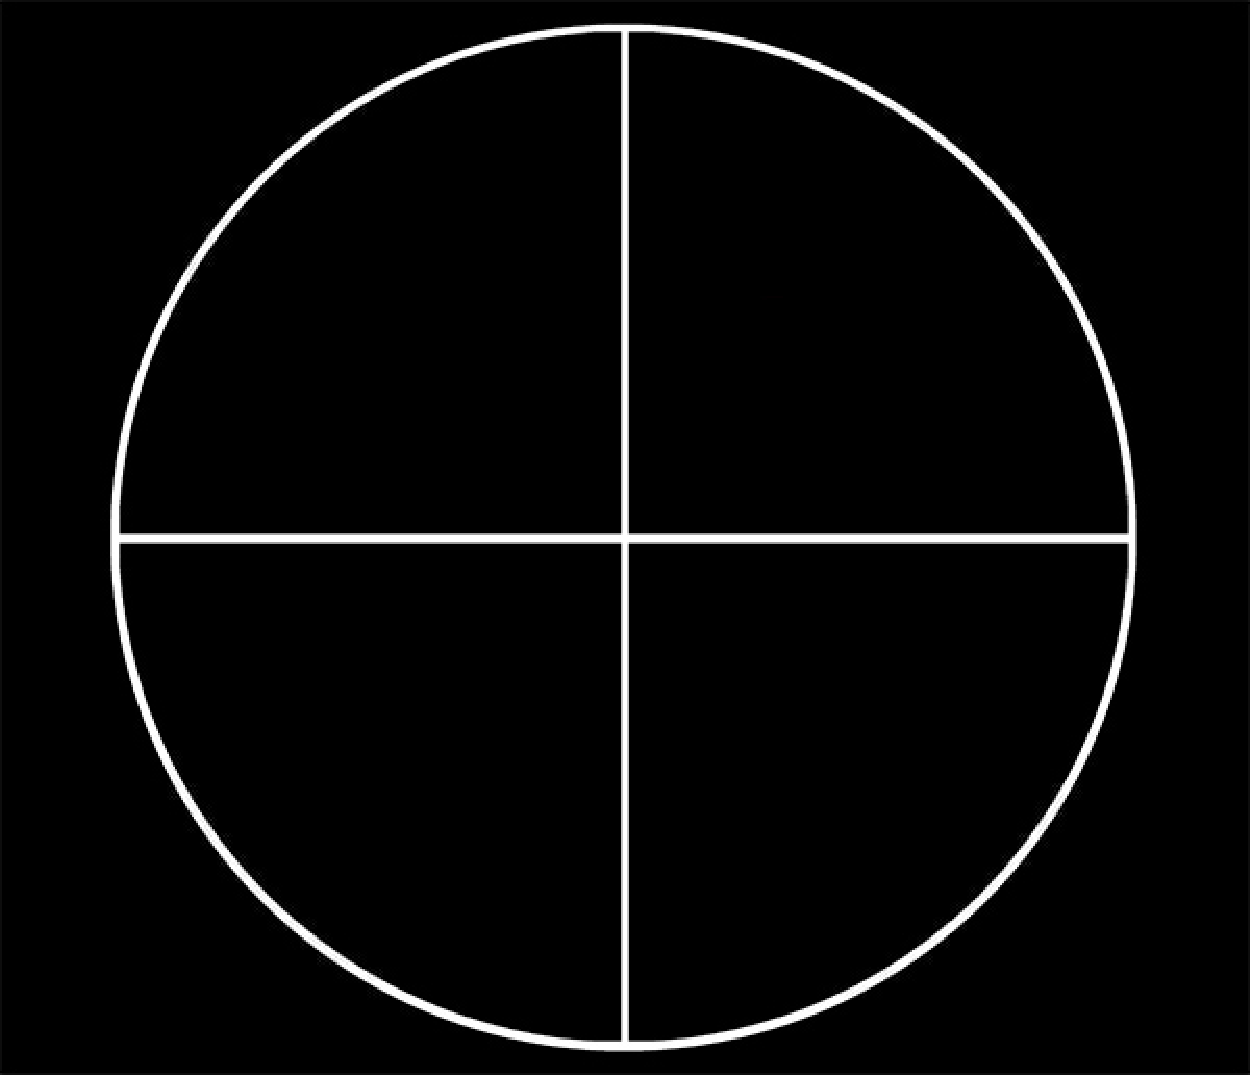
\includegraphics[width=0.3\linewidth]{figures/PDF/Ref_structure.pdf}\\
    \caption{Illustration of a structure based on pre-defined reference key points.}
    \label{fig:keypoint structure}
\end{figure}

\noindent With the key points and its corresponding matches, the homography can now be calculated to finally warp the image to the pre-defined reference points, thus completing the image registration.\\

\noindent Lastly, the elliptical projection of the agar plate, as illustrated in \textit{Figure \ref{fig:method projection}}, needs to be considered to improve the perspective accuracy in the more extreme cases. Since the goal is to produce a flat projection of the agar plate, additional iterations of the whole process will be applied to cope with any perspective distortion.

\begin{figure}[H]
    \centering
    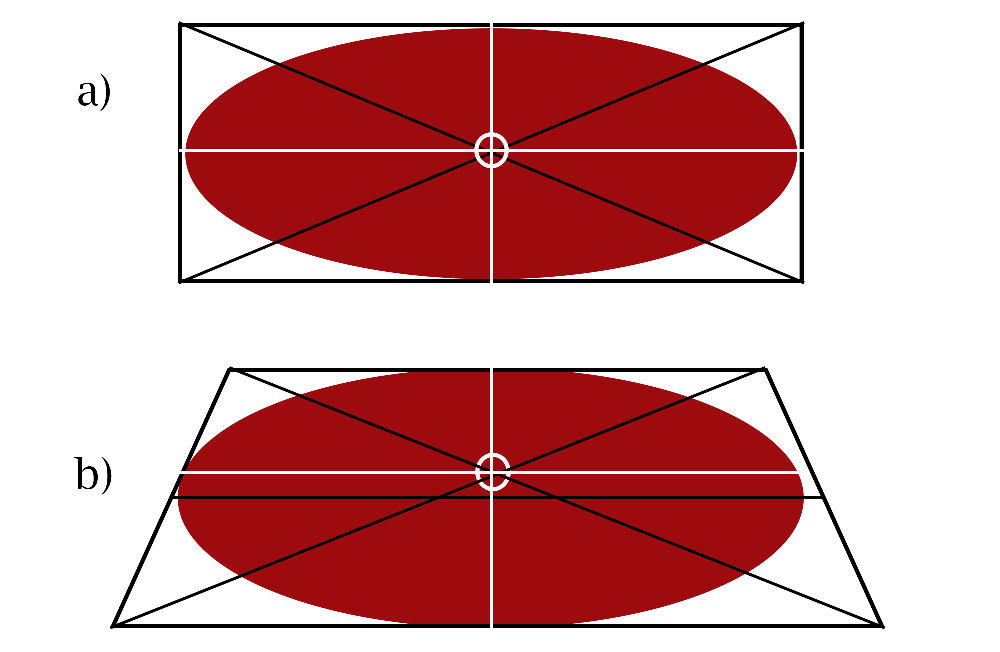
\includegraphics[width=0.5\linewidth]{figures/PDF/Ellipse_projection.pdf}\\
    \caption{a) Flat ellipse. b) Foreshortened circle (spatial illusion).}
    \label{fig:method projection}
\end{figure}

%\color{red} Should we write matches or descriptors? What is the difference? \color{black}


\section{Evaluation}
The approach of this thesis is to evaluate if a combination of image processing techniques can be used to solve the problem description. The thesis problem is assumed to be solved if the criteria in \textit{Section 1.3} are fulfilled. Therefore, the basis of evaluation for this method is to examine if the workflow, shown in \textit{Figure \ref{fig:method workflow}}, can produce results that fulfill the criteria. 


%%%%%%%%%%%%%%%%%%%%%%%%%%%%%%%%%%%%%%%%%%%%%%%%%%%%%%%%%%%%%%%%%%%%%%
%%% lorem.tex ends here

%%% Local Variables: 
%%% mode: latex
%%% TeX-master: "demothesis"
%%% End:
